\chapter{Using a Do file}
\graphicspath{ {./Lab00HowTo/howTo30 Using Do Files/Fig} }


\hypertarget{objective}{%
\section{\texorpdfstring{Objective }{Objective }}\label{objective}}

The objective of this lab note is to help you understand the syntax and
purpose of a DO file.

\textbf{Setting up simulations}

I find setting up the testbench waves to be a pain, especially when you
are making a lot of mistakes and need to rerun your simulation multiple
times; each time setting up the waveforms. In order to simplify the
process of setting up the waveforms, you can write a script files that
performs the waveform setup and then call the script file inside
ModelSim. The script file is called a ``do'' file. They are very easy to
make and will save you time. If a do file is provided to you, you will
most likely need to edit it because your signal names may be different.

In the discussion below I have used two placeholders:
\textless labName\textgreater{} is the name of your testbench module.
\textless projectDirectory\textgreater{} is the system path to your
Verilog files corresponding to your project.

\begin{itemize}
\item
  If provided, download
  ``\textless labName\textgreater\_tbWaveSetup.do'' into the:
  \textless projectDirector\textgreater\textbackslash simulation\textbackslash modelsim
\item
  If a do file is not created, you can use the template provided in
  Listing 1 as a starting point to make one for yourself. Make sure to
  put the do file in the directory:
  \textless projectDirector\textgreater\textbackslash simulation\textbackslash modelsim
\item
  Open \textless labName\textgreater\_tbWaveSetup.do file using Notepad.
  The syntax is pretty straight forward and corresponds to the text
  displayed in the ModelSim console window when you add or modify
  waveforms.
\item
  From Quartus, you need to:

  \begin{itemize}
  \item
    Make sure that your testbench is the top-level. Do this in the
    Project Navigator, select File view and then right click on the file
    testbench and select ``Set As Top Level Entity''
  \item
    Launch the simulation. Do this by selecting Tools -\textgreater{}
    Run Simulation Tool -\textgreater{} RTL Simulation
  \item
    This will launch Model Sim for your testbench
  \end{itemize}
\item
  From Model Sim, you need to:

  \begin{itemize}
  \item
    Maximize the Model Sim window -- this makes it easier to see all the
    subwindows.
  \item
    In the library subwindow, open the \textbf{work} library
  \item
    Right click on your testbench and select Simulate
  \item
    In the console area of ModelSim (shown in the image below) type:
  \end{itemize}
\end{itemize}

\begin{quote}
VSIM 3\textgreater{} do
\textless projectName\textgreater\_tbWaveSetup.do

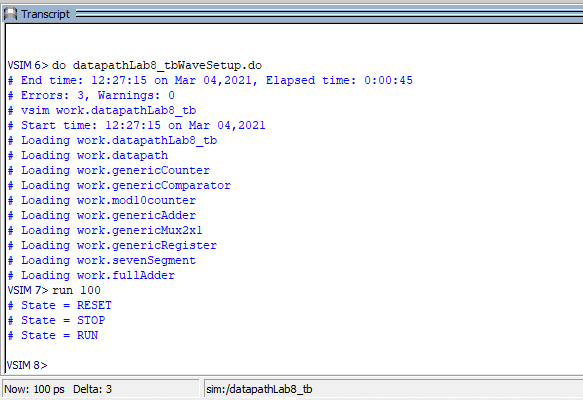
\includegraphics[width=3.02135in,height=2.07297in]{image1.png}
\end{quote}

\begin{itemize}
\item
  You can type ``run \textless time\textgreater'' in this area (as
  shown) to simulate some amount of time. I found this VERY handy when
  debugging my Verilog code.
\item
  Also note that the console has tab completion. This allows you to type
  the first few characters of a command/filename and press Tab to fill
  in the rest of the command/filename. If there is more than one choice,
  the command/filename will be completed up to the ambiguity.
\end{itemize}

\hypertarget{example-do-file-for-hilow-module}{%
\section{\texorpdfstring{Example do file for hiLow Module:
}{Example do file for hiLow Module: }}\label{example-do-file-for-hilow-module}}

\begin{itemize}
\item
  Run the testbench for the hiLow module provided on Canvas. Produce a
  timing diagram with the following characteristics. Zoom to fill the
  available horizontal space with the waveform. Color inputs green and
  outputs red. Order the traces from top to bottom as

  \begin{itemize}
  \item
    t\_seedSwitch unsigned green trace
  \item
    t\_guessSwitch unsigned green trace
  \item
    t\_playSwitch unsigned green trace
  \item
    t\_randBut default green trace
  \item
    t\_hiLowBut default green trace
  \item
    \textless LFSR output\textgreater{} unsigned yellow
  \item
    t\_randNum hex red trace
  \item
    t\_randDisp hex red trace
  \item
    t\_hiLowSeg hex red trace
  \item
    t\_greenLEDs default red trace
  \end{itemize}
\end{itemize}

\begin{itemize}
\item
  The do file for this testbench is shown in Listing 1. From top to
  bottom the sections are as follows.

  \begin{itemize}
  \item
    Any line that starts with a ``\#'' is a comment. The URL is a
    complete reference for do file syntax.
  \item
    The restart command resets the simulation. I included this because I
    sometimes like to rerun the same simulation multiple times. This
    isn't particularly useful for combinational logic circuits.
  \item
    The delete wave command removes any waveforms that may have been
    added previously. Again, I included this because I sometimes like to
    rerun the same simulation multiple times
  \item
    The add wave command puts a signal into the waveform viewing area.
    There are two parameters included which you will find helpful.

    \begin{itemize}
    \item
      Radix changes what base the waveform value is displayed.
    \item
      Color changes the color that the waveform is displayed.
    \end{itemize}
  \end{itemize}
\item
  Once you have created the do file, you call it by running it from the
  console area using the do command discussed previously.
\item
  You can advance the simulation time using the run command discussed
  previously.
\end{itemize}

\end{document}
